\subsection{问题四：波动电价下的规划}\label{sec:q4}
\subsubsection{价格信息与两种决策频率}
问题四采用附件四的实时波动电价。价格变化会影响哪些时段适合购电和储能，因此需要根据预测价格重新制定计划，再按实际价格计算支出。未来电价在决策时尚未知晓，预测控制与预先知道全部价格时的表现存在差别，相关动态价格研究也讨论了这一问题\upcite{perez2023hem}。

本文将“交易时刻电价”解释为对应交付区间的实际价格$p_{d,t}$，用于交付结算。沿用问题三的交易变量，记$\widehat p^{(s)}_{d,t}$为时刻$s$基于已有信息预测的未来电价。问题4-2在$s=0$制定全天固定计划；问题4-3在$s\in\{0,36,72,108\}$进行滚动规划，并沿用光伏预报融合及最终净调整合约。

两种策略采用相同的设备参数、十分钟步长及储能反馈规则，实际储电量均随每日运行连续传递。

\subsubsection{费用目标与价格预测}
问题4-2和4-3的实际购电费用分别为
\begin{equation}
 C_{4-2}=\sum_{d,t}p_{d,t}(g_{d,t}+5e_{d,t}),
\end{equation}
\begin{equation}
\begin{aligned}[b]
 C_{4-3}=\sum_{d,t}p_{d,t}\bigl[&g_{d,t}
 +1.5(q_{d,t}-g_{d,t})_+\\
 &+0.5(g_{d,t}-q_{d,t})_++5e_{d,t}\bigr].
\end{aligned}\label{eq:q4-bill}
\end{equation}
费用均统计2—12月，并按实际价格计算。制定计划时，用预测价格代替尚未知晓的未来价格，零时和日内分别求解
\begin{equation}
 \min\sum_{t=0}^{143}\widehat p^{(0)}_{d,t}g_{d,t},
 \qquad
 \min\sum_{t=s}^{143}1.5\widehat p^{(s)}_{d,t}
       (q^{(s)}_{d,t}-g_{d,t}).\label{eq:q4-objectives}
\end{equation}
第二个目标用于问题4-3的$s>0$。两项目标决定当次购电安排，最终费用则由实际交付电量和价格核算。

电价预测考虑周周期特征。当$d\ge7$时，选取此前最多四个与目标日星期相同的日期，对同一时刻电价进行衰减加权：
\begin{equation}
 \overline p_{d,t}=
 \frac{\sum_{k=1}^{K_d}0.55^{k-1}p_{d-7k,t}}
      {\sum_{k=1}^{K_d}0.55^{k-1}},
 \qquad K_d=\min\{4,\lfloor d/7\rfloor\}.
\end{equation}
历史不足一周时，取此前最多7天，以0.8的衰减系数加权。零时取$\widehat p^{(0)}_{d,t}=\max(\overline p_{d,t},0.001)$。问题4-3在日内根据最近18段实际价格的均值修正预测水平，使用式\eqref{eq:clip}将修正比例限制在$[0.5,1.5]$。记
\begin{equation}
 r^{p}_{d,s}=\operatorname{clip}\!\left(
 \frac{\frac1{18}\sum_{j=s-18}^{s-1}p_{d,j}}
      {\max\left(\frac1{18}\sum_{j=s-18}^{s-1}\overline p_{d,j},0.01\right)},
 0.5,1.5\right),
\end{equation}
由此得到剩余时段的价格预测：
\begin{equation}
 \widehat p^{(s)}_{d,t}=\max\{0.001,r^{p}_{d,s}\overline p_{d,t}\},
 \qquad t\ge s,\quad d\ge1.\label{eq:price-update}
\end{equation}
比例截断可避免历史均值很小时产生过大的修正，价格下限保证目标系数为正。首日各发布时间均采用附件一的固定价格，用于1月初始化；从随后日期起，按已完成区间的观测计算预测和修正比例。

\subsubsection{分条约束与汇总模型}
\textbf{a) 物理约束。}每次规划仍满足风险净负荷下的能量平衡、储能效率、功率和安全库存限制。价格改变目标系数，不改变物理守恒关系。

\textbf{b) 库存衔接。}零时从实际$S_{d,0}$开始，日内从实际$S_{d,s}$开始，预测日末恢复目标均为6000\,kWh。实际跨日运行不重置库存。

\textbf{c) 交易频率与原计划下界。}问题4-2全天$q_t=g_t$；问题4-3在三次允许时刻修改未交付量，且$q^{(s)}_t\ge g_t$。实际和预测价格均为正，故问题三关于保留原计划量更有利的论证仍适用。

\textbf{d) 可用信息与实际结算。}预测价格、净负荷和本次计划均由$\mathcal H_{d,s}$确定；之后观测到的$p_{d,t}$用于结算对应交付段的费用，已执行决策保留原记录。

为统一两种频率，令允许的发布时间集合为$\mathcal S$；零时取$\ell^{(0)}_t=0$、$\kappa_0=1$，日内取$\ell^{(s)}_t=g_t$、$\kappa_s=1.5$。每次求解
\begin{equation}
\begin{aligned}[b]
 (\mathrm P_4^{(s)})\quad\min\quad&
  \sum_{t=s}^{143}\kappa_s\widehat p^{(s)}_{d,t}
       (q^{(s)}_t-\ell^{(s)}_t),\\
 \mathrm{s.t.}\quad&q^{(s)}_t+\widehat b_t
       =\widetilde N^{(s)}_{d,t}+\widehat c_t+\widehat w_t,\\
 &\widehat S_{t+1}=\widehat S_t+0.9\widehat c_t-\widehat b_t/0.9,\\
 &0\le\widehat c_t,\widehat b_t\le5000/6,\quad
   q^{(s)}_t\ge\ell^{(s)}_t,\quad\widehat w_t\ge0,\\
 &1200\le\widehat S_t\le10800,\quad
   \widehat S_s=S_{d,s},\quad\widehat S_{144}\ge6000.
\end{aligned}\label{eq:q4-summary}
\end{equation}
零时求得的计划为$g_t=q^{(0)}_t$。问题4-2取$\mathcal S=\{0\}$，问题4-3取$\mathcal S=\{0,36,72,108\}$；区间约束作用于$t=s,\ldots,143$，库存边界还包括144。模型据此统一表示两种规划频率。

\subsubsection{求解与结算步骤}
沿用问题二、三的候选集合，按1月15—31日实际费用选参。问题4-2选得$\alpha=0.80$，问题4-3选得$(\lambda,\alpha)=(0.50,0.65)$。问题4-3的1月热启动固定使用纯附件三预测、0.80分位及三次调整，2月起采用所选参数。

按时间先后运行以下步骤：
\begin{enumerate}
 \item 零时继承真实库存，以过去日期分别预测负荷、光伏和价格；构造风险净负荷。
 \item 用预测价格作为目标系数求解$(\mathrm P_4^{(0)})$，锁定原计划并保存预测曲线。
 \item 问题4-2按固定计划运行；问题4-3在各发布时间利用新预报及最近观测更新负荷、光伏和价格预测，求解剩余时段模型。
 \item 交付时根据当段实际净负荷执行充放电，放电后的缺口由紧急购电补足。
 \item 用该段实际价格结算原计划、最终净调整和紧急购电，更新实际库存。
 \item 日末传递库存，2月起累计正式费用；从逐段数组分别重算全年和指定日期账单。
\end{enumerate}

为检查信息使用顺序，将未来实际价格替换后重新计算，确认当前预测和计划不受影响。历史误差也按日期和发布时间读取，只有已完成区间的误差参与当前修正。

\subsubsection{波动电价结果及比较}
问题4-2总费用为\PaperValue{q4-2-cost}\,元，问题4-3为\PaperValue{q4-3-cost}\,元，日内方案节省\PaperValue{q4-3-saving}\,元，降幅\PaperValue{q4-3-saving-percent}\%。表\ref{tab:q4-comparison}给出费用与电量分解。
\par
\begin{table}[!htbp]
\centering
\caption{波动电价下两种策略的结果（2—12月）}\label{tab:q4-comparison}
\normalsize
\begin{tabular}{lrr}
\toprule
\multicolumn{1}{c}{指标} & \multicolumn{1}{c}{问题4-2} & \multicolumn{1}{c}{问题4-3} \\
\midrule
原计划费/元 & 14,032,328.84 & 13,366,608.69 \\
调整费/元 & 0.00 & 550,605.94 \\
紧急费/元 & 643,516.03 & 127,670.62 \\
总费用/元 & 14,675,844.87 & 14,044,885.25 \\
常规购电/kWh & 21,708,087.29 & 21,192,613.91 \\
紧急购电/kWh & 101,425.76 & 24,227.41 \\
未利用电量/kWh & 2,632,806.82 & 2,009,834.69 \\
发生紧急购电的天数 & 108 & 134 \\
期初储电量/kWh & 6,864.27 & 7,114.54 \\
期末储电量/kWh & 6,263.02 & 5,997.11 \\
\bottomrule
\end{tabular}
\end{table}
\par

\FloatBarrier
日内方案降低了原计划费和紧急费，计入新增550605.94元调整费后，总支出仍较低。紧急电量由101425.76\,kWh降至24227.41\,kWh，发生天数却由108增至134。与固定电价下相同，紧急购电的总规模缩小，但分布在更多日期。

图\ref{fig:q4-months}给出逐月费用及紧急电量，便于在相同月份和实际电价下比较两种策略。固定电价与波动电价的费用差还包含价格水平、购电安排和库存变化，解释这一差异时需同时考虑这些因素。
\begin{figure}[!htbp]
 \centering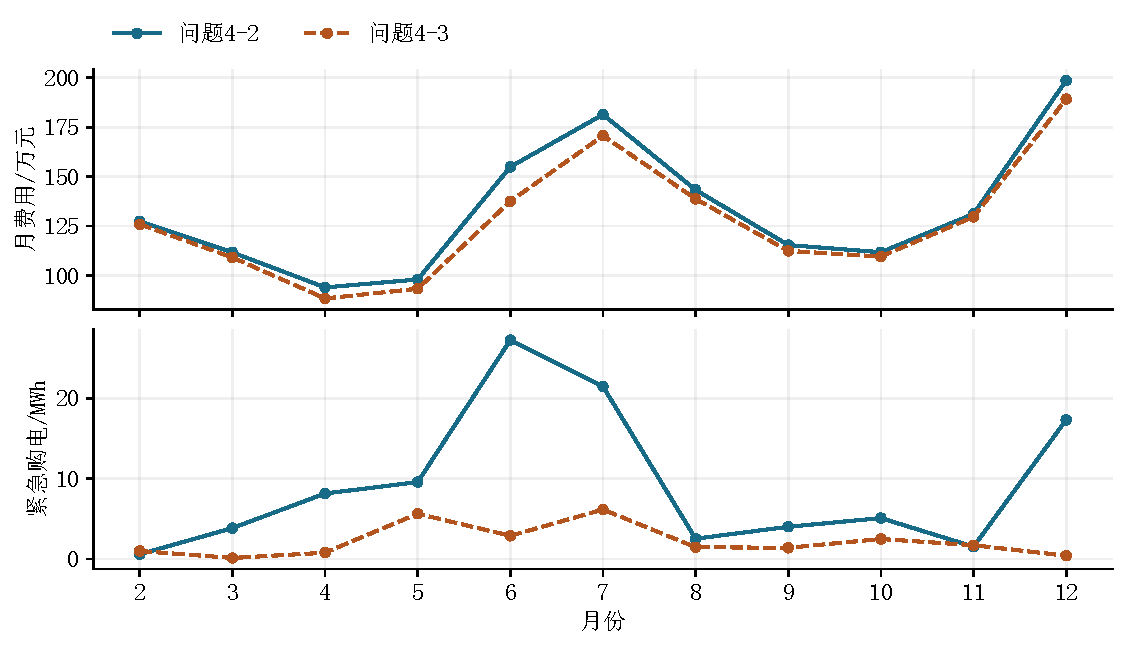
\includegraphics[width=\textwidth]{../outputs/figures/paper-q4-months.pdf}
 \caption{波动电价下各月费用与紧急购电量}\label{fig:q4-months}
\end{figure}
\FloatBarrier
指定日期费用列于表\ref{tab:q4-days-summary}。在9月23日，允许调整后的全天总费从49762.23元降至45799.34元；12月21日两种方案费用均较高。下一小节分别展示9月23日的购电与储能；其余日期、紧急事件及账单见附录\ref{app:q4-2-days}、\ref{app:q4-3-days}，完整策略保存在\texttt{result4-2.xlsx}、\texttt{result4-3.xlsx}。
\par
\begin{table}[!htbp]
\centering
\caption{波动电价下指定日期费用（2025年，元）}\label{tab:q4-days-summary}
\normalsize
\begin{tabular}{lrrr}
\toprule
\multicolumn{1}{c}{日期} & \multicolumn{1}{c}{问题4-2} & \multicolumn{1}{c}{问题4-3} & \multicolumn{1}{c}{日内方案节省} \\
\midrule
03-20 & 42,627.22 & 42,600.22 & 27.00 \\
06-21 & 19,640.47 & 18,336.05 & 1,304.42 \\
09-23 & 49,762.23 & 45,799.34 & 3,962.89 \\
12-21 & 75,769.21 & 72,885.14 & 2,884.07 \\
\bottomrule
\end{tabular}
\end{table}
\par


在共同热启动下比较光伏来源，融合方案比纯历史基准少支出122075.92元，也比单用附件三更省费，完整结果见附录\ref{app:parameter-checks}表\ref{tab:q4-3-forecast}。各预测方法分别选择参数，因此费用差反映了预测方法与相应控制参数共同作用的结果。
\FloatBarrier

\subsubsection{代表日期的购电与储能结果}
\textbf{a) 问题4-2：零时固定计划。}以下按题面表1、表2列出9月23日。购电表给出常规计划电量及按实际交付价格结算的常规费；电量为kWh，费用为元。
% Generated by scripts/build_paper_tables.py; do not edit by hand.
2025.9.23的购电和储能结果分别见表\ref{tab:q4-2-2025-09-23-purchase}和表\ref{tab:q4-2-2025-09-23-storage}。

\par
\begin{table}[!htbp]
\centering
\caption{微网在指定时间段的购电量及全天的购电量和购电费（2025.9.23）}\label{tab:q4-2-2025-09-23-purchase}
\normalsize
\begin{tabular}{lrlrlr}
\toprule
\multicolumn{1}{c}{时间段} & \multicolumn{1}{c}{购电量} & \multicolumn{1}{c}{时间段} & \multicolumn{1}{c}{购电量} & \multicolumn{1}{c}{时间段} & \multicolumn{1}{c}{购电量} \\
\midrule
10:00--10:10 & 0.00 & 12:00--12:10 & 499.87 & 14:00--14:10 & 0.00 \\
16:00--16:10 & 531.67 & 18:00--18:10 & 775.50 & 20:00--20:10 & 0.00 \\
\multicolumn{2}{c}{全天购电量} & 68,171.89 & \multicolumn{2}{c}{全天购电费} & 44,011.52 \\
\bottomrule
\end{tabular}
\end{table}
\par


\par
\begin{table}[!htbp]
\centering
\caption{储能设备在指定时间段的充放电量及0:00和24:00的储电量（2025.9.23）}\label{tab:q4-2-2025-09-23-storage}
\normalsize
\begin{tabular}{lrrlrr}
\toprule
\multicolumn{1}{c}{时间段} & \multicolumn{1}{c}{充电量} & \multicolumn{1}{c}{放电量} & \multicolumn{1}{c}{时间段} & \multicolumn{1}{c}{充电量} & \multicolumn{1}{c}{放电量} \\
\midrule
0:00--4:00 & 4,837.74 & 54.89 & 4:00--8:00 & 801.19 & 6,062.63 \\
8:00--12:00 & 5,459.91 & 1,896.62 & 12:00--16:00 & 4,418.80 & 560.16 \\
16:00--20:00 & 79.59 & 5,673.19 & 20:00--24:00 & 5,585.42 & 2,617.77 \\
\multicolumn{2}{c}{0:00储电量} & 5,901.66 & \multicolumn{2}{c}{24:00储电量} & 6,226.87 \\
\bottomrule
\end{tabular}
\end{table}
\par


\FloatBarrier

\textbf{b) 问题4-3：日内调整。}购电表分别展示零时原计划与最终常规购电，费用口径与问题三相同，均按实际交付价格核算；储能表列实际运行结果。指定日的初始库存承接前日，两组方案均从全年起点6000\,kWh连续运行至该日。
% Generated by scripts/build_paper_tables.py; do not edit by hand.
2025.9.23的购电和储能结果分别见表\ref{tab:q4-3-2025-09-23-purchase}和表\ref{tab:q4-3-2025-09-23-storage}。

\par
\begin{table}[!htbp]
\centering
\caption{微网在指定时间段的购电量及全天的购电量和购电费（2025.9.23）}\label{tab:q4-3-2025-09-23-purchase}
\normalsize
\begin{tabular}{lrlrlr}
\toprule
\multicolumn{6}{c}{零时原计划} \\
\multicolumn{1}{c}{时间段} & \multicolumn{1}{c}{购电量} & \multicolumn{1}{c}{时间段} & \multicolumn{1}{c}{购电量} & \multicolumn{1}{c}{时间段} & \multicolumn{1}{c}{购电量} \\
\midrule
10:00--10:10 & 0.00 & 12:00--12:10 & 401.83 & 14:00--14:10 & 0.00 \\
16:00--16:10 & 520.87 & 18:00--18:10 & 763.88 & 20:00--20:10 & 0.00 \\
\multicolumn{2}{c}{全天购电量} & 65,294.82 & \multicolumn{2}{c}{全天购电费} & 42,202.79 \\
\addlinespace
\multicolumn{6}{c}{最终常规购电} \\
时间段 & 购电量 & 时间段 & 购电量 & 时间段 & 购电量 \\
10:00--10:10 & 0.00 & 12:00--12:10 & 401.83 & 14:00--14:10 & 0.00 \\
16:00--16:10 & 520.87 & 18:00--18:10 & 793.71 & 20:00--20:10 & 0.00 \\
\multicolumn{2}{c}{全天购电量} & 67,099.79 & \multicolumn{2}{c}{全天购电费} & 44,903.59 \\
\bottomrule
\end{tabular}
\end{table}
\par


\par
\begin{table}[!htbp]
\centering
\caption{储能设备在指定时间段的充放电量及0:00和24:00的储电量（2025.9.23）}\label{tab:q4-3-2025-09-23-storage}
\normalsize
\begin{tabular}{lrrlrr}
\toprule
\multicolumn{1}{c}{时间段} & \multicolumn{1}{c}{充电量} & \multicolumn{1}{c}{放电量} & \multicolumn{1}{c}{时间段} & \multicolumn{1}{c}{充电量} & \multicolumn{1}{c}{放电量} \\
\midrule
0:00--4:00 & 4,267.49 & 194.62 & 4:00--8:00 & 996.54 & 6,251.03 \\
8:00--12:00 & 5,281.76 & 1,896.62 & 12:00--16:00 & 5,288.36 & 509.61 \\
16:00--20:00 & 111.95 & 5,255.66 & 20:00--24:00 & 5,591.15 & 3,287.90 \\
\multicolumn{2}{c}{0:00储电量} & 6,169.40 & \multicolumn{2}{c}{24:00储电量} & 6,224.67 \\
\bottomrule
\end{tabular}
\end{table}
\par


\FloatBarrier

\subsubsection{价格与参数灵敏度检验}
先检验预测峰谷价差的影响。记$m_{d,s}$为本次剩余时段的预测价格均值，将价格曲线改为
\begin{equation}
 \widehat p^{(s,\theta)}_{d,t}
 =\max\{0.001,m_{d,s}+(1+\theta)
       (\widehat p^{(s)}_{d,t}-m_{d,s})\},\qquad
 \theta\in\{-0.2,0,0.2\}.\label{eq:price-sensitivity}
\end{equation}
负扰动缩小预测峰谷差，正扰动扩大预测峰谷差，均根据当时可得的预测曲线计算。各组采用相同负荷、光伏、实际结算价、控制参数及1月热启动，从2月起按扰动后的预测重新规划并连续运行。表\ref{tab:q4-price-sensitivity}列出实际费用和年末库存。
\par
\begin{table}[!htbp]
\centering
\caption{预测价差幅度扰动（共同热启动，2—12月）}\label{tab:q4-price-sensitivity}
\normalsize
\begin{tabular}{lrrrr}
\toprule
\multicolumn{1}{c}{方案} & \multicolumn{1}{c}{$\theta$} & \multicolumn{1}{c}{总费用/元} & \multicolumn{1}{c}{较主方案增费/元} & \multicolumn{1}{c}{期末储电量/kWh} \\
\midrule
问题4-2 & -0.2 & 14,674,479.32 & -1,365.55 & 6,263.02 \\
问题4-2 & 0 & 14,675,844.87 & 0.00 & 6,263.02 \\
问题4-2 & +0.2 & 14,683,290.13 & 7,445.26 & 6,263.02 \\
问题4-3 & -0.2 & 14,042,823.76 & -2,061.48 & 5,997.11 \\
问题4-3 & 0 & 14,044,885.25 & 0.00 & 5,997.11 \\
问题4-3 & +0.2 & 14,061,149.66 & 16,264.42 & 5,997.11 \\
\bottomrule
\end{tabular}
\end{table}
\par

\FloatBarrier
扩大预测价差20\%时，两种策略分别增费7445.26元和16264.42元；缩小20\%时分别减费1365.55元和2061.48元。四组扰动与各自主方案的期末库存相同，可在相同储备水平下比较支出。本次范围内总费变化均小于0.12\%，日内调整方案仍更省费。该检验说明策略对价差幅度的小范围变化较稳定，峰谷时刻错位和极端电价的影响仍待检验。

另作已知未来价格的对照，直接用实际价格规划，问题4-2与4-3费用分别为\PaperValue{q4-2-oracle}\,元和\PaperValue{q4-3-oracle}\,元。该对照使用了执行时无法提前获得的信息，热启动和后续库存也随之变化，因此仅作为事后参考，尚不足以给出随机全年问题的严格下界。实际预测策略的零时平均绝对价格误差约为0.04456元/kWh，其费用影响需结合购电量和储能动作分析。

风险参数的选择结果见附录\ref{app:parameter-checks}表\ref{tab:q4-calibration}。按1月15—31日费用评分，问题4-3固定融合权重0.50，固定计划和日内调整分别在0.80和0.65处取得候选中的最低费用。提高分位可减少缺口，也会增加提前购电支出；这里的选择仅依据1月评分。
\FloatBarrier
跨月实验按训练先于评价的顺序\upcite{cerqueira2020evaluation}，每月根据上月费用重选参数，各组从共同4月1日库存连续运行。问题4-3的逐月选参方案比固定参数多支出16320.66元，9个月中仅1个月更省，说明频繁重选在本年度没有改善累计费用。完整账单与库存见附录\ref{sec:rolling}。

在相同信息、参数及热启动条件下，将储能控制换成确定性滚动反馈\upcite{wytock2017dem}，问题4-2和4-3分别增费33995.79元、213489.58元，期末库存与原反馈相同。该配置尚未估计跨日库存价值，结果说明它在本组设置下未优于原反馈；进一步改进需同时考虑次日的用电需求。模型及费用分解见附录\ref{sec:feedback}。
\label{end:q4}
